\documentclass[a4paper,10pt]{article}
\usepackage[hidelinks]{hyperref}
\def\UrlBreaks{\do\/\do-} % breaks long url in references
\usepackage{graphicx}
\usepackage[english]{babel}
\usepackage{listings}
\usepackage[labelfont=it,textfont={it},singlelinecheck=on,justification=centering]{caption}
\usepackage{amsmath}
\usepackage{float}
%\usepackage{draftwatermark}
%\SetWatermarkLightness{0.97}
%\DeclareGraphicsExtensions{.pdf,.png,.jpg}
\begin{document}
\lstset{basicstyle=\ttfamily\footnotesize,breaklines=true}
\lstset{numbers=left, numberstyle=\tiny, stepnumber=1, numbersep=5pt}
\lstset{language=TeX}
%\SetWatermarkScale{8}

\title{\textbf{Storj\\A Peer-to-Peer Cloud Storage Network}}
\author{Shawn Wilkinson (shawn@storj.io)\\
\\Contributors:\\ 
Tome Boshevski (tome@storj.io), Josh Brandoff (josh@storj.io),\\ 
and Vitalik Buterin (v@buterin.com)}
\maketitle
\begin{abstract}
A peer-to-peer cloud storage network implementing end-to-end encryption would allow users to transfer and share data without reliance on a third party data provider. The removal of central controls would eliminate most traditional data failures and outages, as well as significantly increasing security, privacy, and data control. A peer-to-peer network and basic encryption serve as a solution for most problems, but we must offer proper incentivation for users to properly participate in this network. We propose a solution to these additional problems by using a challenge algorithm. In this way we can periodically cryptographically check the integrity and availability of a file, and offer direct rewards to those maintaining the file. In absence of a peer-to-peer network the described methods may be used to allow users to control, migrate, validate their data on 3rd party data providers without the provider having direct access to the data. 
\end{abstract}

\section{Introduction}
Cloud storage on the Internet has come to rely almost exclusively on data providers serving as trusted third parties to transfer and store the data. While the system works well enough in most cases, it still suffers from the inherent weaknesses of the trust-based model. Because end-to-end encryption is non-standard, the traditional cloud is open to a variety of security threats, including man-in-the-middle attacks, malware, and application hacks that expose sensitive and private consumer and corporate data. Furthermore, current cloud storage applications are able to charge large premiums on data storage over their core costs because users have few interoperable and featureful providers to choose from. Moreover, these third party providers may have technical failures that can cause data breaches and unavailability, much to the distress of the users and applications that depend on them. These shortcomings were discussed in greater depth in our previous white paper on MetaDisk \cite{1}.\\

What is needed is a decentralized cloud storage platform that implements end-to-end encryption on a decentralized and open network. This platform must be resistant to attackers who might attempt Sybil attacks and other forms of fraud. Additionally, this network must account for the latency, performance, and downtime of average user computers and dedicated hardware. In our proposed network, cryptographic algorithms would protect data in transit and on devices not controlled by the user. An open market would eliminate the large premiums by allowing all data to be equally traded and moved around the network. Because most internet-connected computers have unused hard drive space, users could sell these resources to the network. Files on this network will be handled by their content, via a hash. The data on the network would be fairly resistant to censorship, tampering, and/or data failures. As long as one copy of the file exists it can be accessed, regardless of whether the original provider is still online.\\

\section{Files as Encrypted Shards}
We identify a shard as an encrypted portion of a file that we would like to store on this network. Splitting the file into shards allows for better data security so that no one farmer will have a complete copy as long as the file being stored is above a standardized shard size. We define a farmer as a user that is leasing his or her hard drive space to the network. We define a standardized shard size as a byte multiple such as 8 MB or 32 MB. These are kept at pre-set sizes to dissuade any attempt to determine what is being stored. Sharding also allows large files to be more manageable as they are distributed throughout the network. 
\\
%insert Figure 1
\begin{figure}[hbt]
\centering
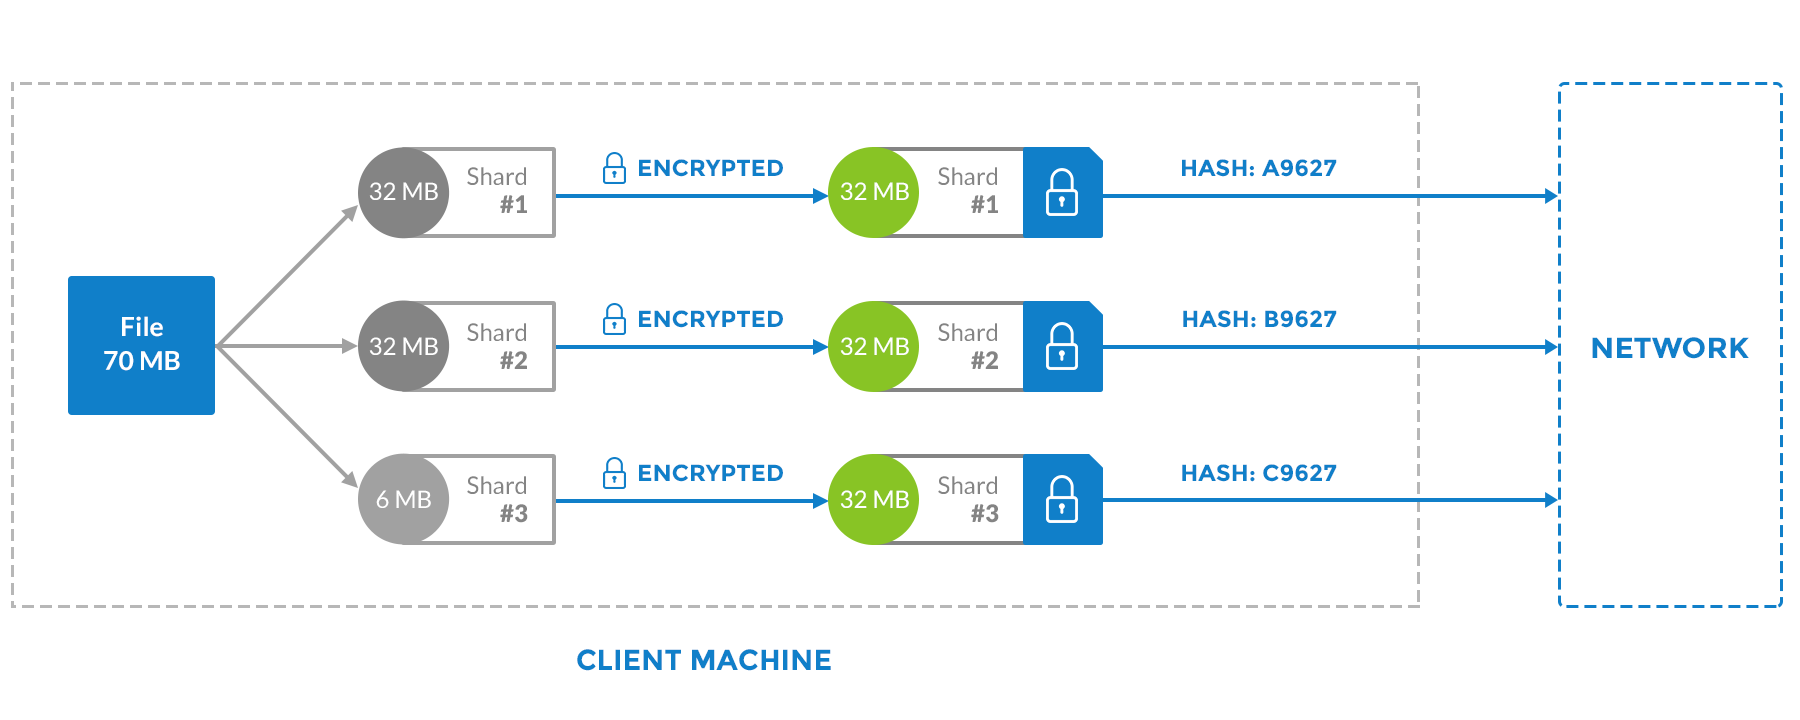
\includegraphics[width=\linewidth]{1}
\caption{Visualizing the Sharding Process}
\end{figure}

\begin{enumerate}
\item File is split into some standard byte-multiple like 32 MB, or multiple smaller files are combined to form a shard. Any extra space is zero filled.
\item Each shard is encrypted convergently or with a user defined method such as with an external encryption key.
\item The shards may be directly transmitted to the network. Shards may be further modified, depending on the file-auditing mechanism.
\end{enumerate}

If necessary, multiple shards can be combined together. This is useful in two situations. First, if the client is storing particularly sensitive or important data, it might be useful to combine their shards with other client’s data or garbage data, in order to disguise their own files. As further described, we use verification and auditing methods on the files, but this creates unnecessary overhead to verify a small document, so it might be worth combining many small files together so they can all be verified at once.



\section{Proof-of-Storage}

Another concern is the integrity and availability of a shard stored on the network. A farmer must be able to prove cryptographically that it has the shard, and has not modified it in any way. We accomplish this via the methods discussed below.
\subsection{Proof-of-Storage via Merkle Audits}

To implement a trustless data storage network, we must provide a method for a client to audit that the data he or she has stored on the network is available and unmodified. We do this through the use of Merkle trees \cite{2} and Merkle proofs. We take a collection of data and generate a Merkle tree as shown in Figure 2:\\

%insert Figure 2
\begin{figure}[hbt]
\centering
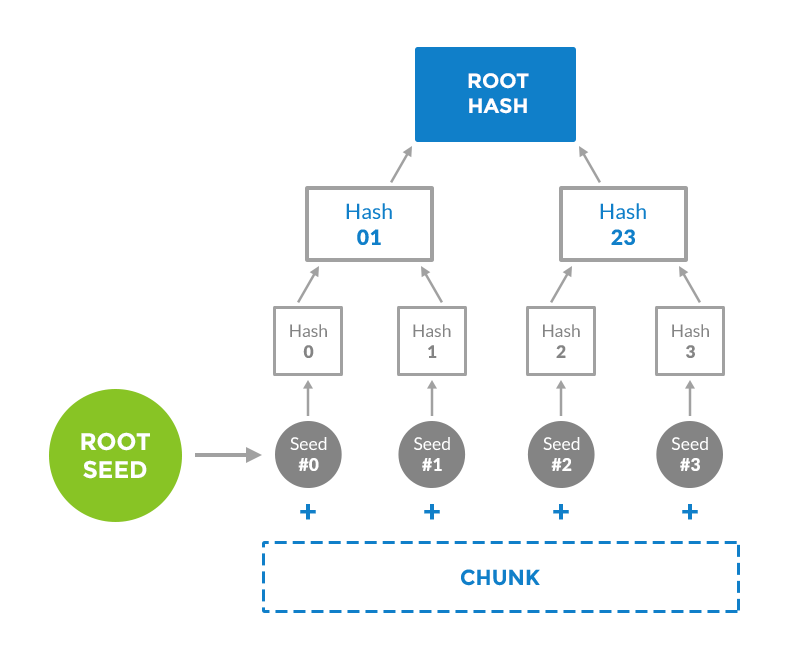
\includegraphics[width=\linewidth]{2}
\caption{Generating a Data Merkle Tree}
\end{figure}

 The leaves of the tree should be 256-byte shards or smaller. Ideally the tree should be larger than the data, so the tree should be generated on the fly instead of stored. An audit of the data on a remote location simply consists of a particular index and a response consisting of the sub-shard located at that index plus a Merkle tree SPV proof. This algorithm has been further described in Secret
Sharing and Erasure Coding \cite{16}. ”  \\


\subsection{Proof-of-Storage via Pre-generated Audits}
We present an alternate method for audits, which requires more overhead but may have some advantages over the previous methods. We do this through a hash challenge, where the client creates a series of seeds (deterministically from a root seed) that can be added to the file and hashed to generate a unique hash answer. We refer to this process as a “heartbeat”. The client generates these hash challenges, builds a Merkle tree \cite{2} and inserts the Merkle root into a Satoshi-style blockchain. It then publishes or gives the Merkle tree, minus the leaves, to the farmer. The client can then periodically issue the seeds to farmers hosting its data, and check if a farmer’s response matches its generated hash answers, by verifying that the hash the farmer responds with is in the Merkle tree. \\

%insert Figure 3
\begin{figure}[hbt]
\centering
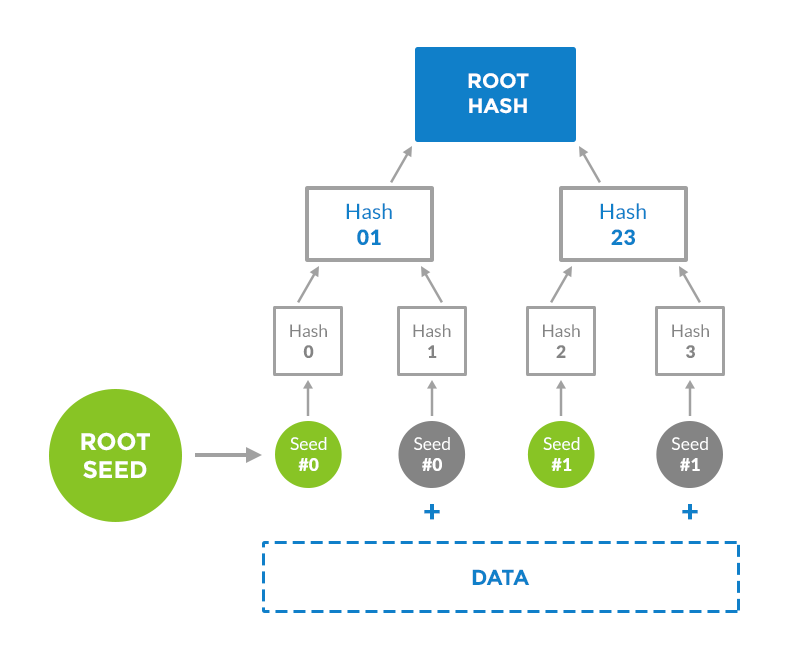
\includegraphics[width=\linewidth]{3}
\caption{Generating a Merkle Root for Some Data}
\end{figure}

The farmer cannot modify or delete the file because he or she will fail the hash challenges, as further described in section 8. By the premises of cryptography and hashing, these heartbeats cannot be brute forced. The client cannot cheat the farmer, because the hash responses can be verified via the Merkle root, which is inserted into a blockchain. In this way we use blockchain backed proof-of-existence \cite{4} \cite{5} to keep either party honest.\\

We generate challenges using 3 different mechanisms: \\

%insert Figure 4
\begin{figure}[hbt]
\centering
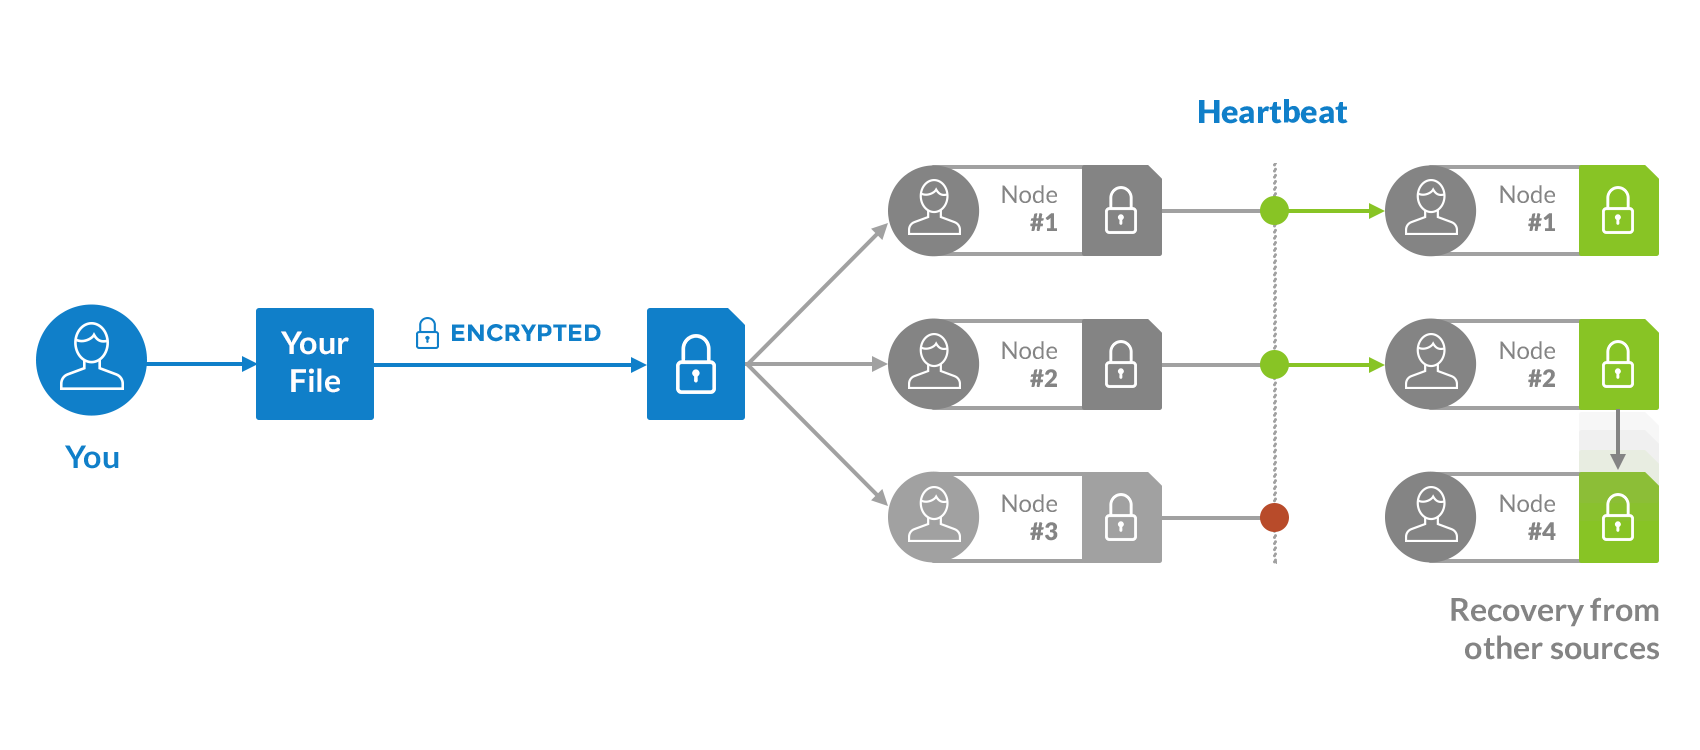
\includegraphics[width=\linewidth]{4}
\caption{Three Methods of Generating Hash Challenges}
\end{figure}

\subsection{Full Heartbeat}
We can use our seed and the full shard to generate our hash response. This verifies full shard integrity, but is extremely I/O-inefficient, and leads to long seek times.
\subsection{Cycle Heartbeat}
A small improvement is where the shard is split into n discrete pieces, and we verify each piece in order until we complete the cycle. This method was first described in part by Filecoin \cite{11}. This is more I/O-efficient, and allows us to fully verify shard integrity after n heartbeats. Unfortunately, it leaves the system open to potential attacks, as an attacker would still be able to complete heartbeats, with only a data integrity of $1/n$.
\subsection{Deterministic Heartbeat}
In this method, we deterministically generate reads on a shard using a root seed passed to us by the client. Using Feistel permutations we can verify data after at most$n+2 \sqrt{n}$ challenges. We add erasure encoding to our heartbeat scheme so that any minor changes to the shard will be detected by the heartbeat, or recovered upon shard retrieval. This is the most efficient method, and by adjusting our parameters we can balance I/O efficiency and file integrity verification.  
\subsection{Mixed Methodology}
Each method has its own advantages and disadvantages. We propose using a combination of these methods. It is recommended that a full heartbeat is used when the file is first uploaded to the network. Cycle heartbeats should be used periodically over a defined timescale. Deterministic heartbeats should be used for all other challenges. In this way, we can benefit from all the advantages offered by each algorithm. 

\section{Proof-of-Redundancy}
Traditional cloud storage companies own or lease servers to store their customers’ files. They use RAID schemes or a multi-datacenter approach to protect the file from physical or network failure. Storj has no central services. File exist in a distributed, virtual, and decentralized network. We can not depend on a farmer to employ the same safety measures against data loss as a traditional cloud storage company. Because of this, we guarantee redundancy by storing shards using an K-of-M erasure encoding scheme with multiple farmers. More specifically we account for redundancy on the network layer rather than the physical layer. We must also provide a solution to the possibility of farmers simply turning off their computers, thus removing the availability of a shard from the network. \\

%insert Figure 5
\begin{figure}[hbt]
\centering
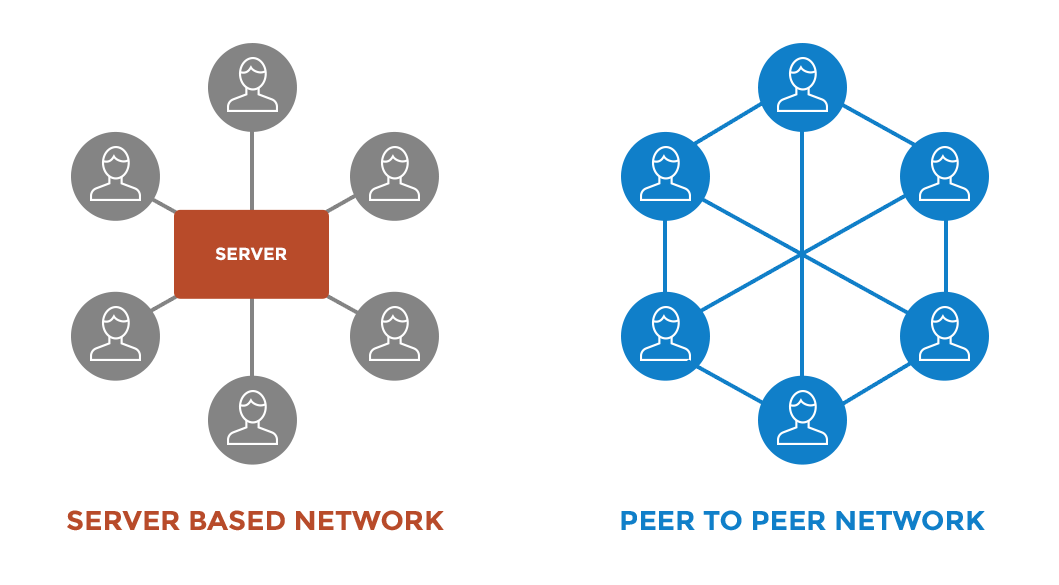
\includegraphics[width=\linewidth]{5}
\caption{Visualizing Audits}
\end{figure}

\subsection{Simple Fault Tolerance}
If a node fails an audit or is unreachable, we initiate a network replication process whereby we take one of the existing copies on the network and transfer it to a new node. Therefore, the network is able to heal itself after each audit.\\

\subsection{Sybil Redundancy Attacks}
Each shard is uniquely encrypted. This means that malicious farmers can’t pretend to have multiple redundant copies of a file when they only have one. We can accomplish this by adding a deterministic salt value before convergently encrypting the shard. Even if the decryption key is known for a particular file, the malicious farmers will not be able to complete the audits for the shards they have not been assigned. In this way we can prove redundancy for a particular shard, because each redundant copy is unique.\\

\subsection{K-of-M Erasure Encoding}
We use a K-of-M erasure encoding scheme to make sure shards of files are available. The client may choose K and M to achieve a balance of file robustness and costs. The Calculations section more statistically describes file robustness. Erasure encoding also provides protections against the hostage bytes and modified bytes described in the Attacks section.\\

\subsection{Redundancy Scaling}
Ultimately the user and application are in control of redundancy through K-of-M erasure encoding parameters and distribution. For simple data storage, users may choose a recommended setting that may have their data evenly distributed among 3-4 farmers. This should be sufficient for basic fault tolerances. If the data is particularly important, users may distribute the data to 500 farmers, which should protect that data against Armageddon and acts of God. K-of-M schemes also will affect robustness of the data. 

\section{Blockchain}
For the network to be able to achieve consensus on file location and integrity, we use Satoshi-style blockchains \cite{3}. As the blockchain is a public ledger, it is an excellent tool for retrieving accurate information, and as the ultimate mechanism to resolve disputes and dissuade attacks. To use a basic analogy, it is easy to steal a cookie from a cookie jar in a secluded area, but it is hard to do so when the jar is instead located in the middle of a public square, being observed by thousands of people. By using a blockchain as a distributed data store, we can build off of an established and time-tested distributed consensus mechanism. We do not store any files in the blockchain, but rather file metadata. In essence, we store the file hash, the network locations of the copies of the shards, and Merkle roots. The specifics and scalability of this method are described in the MetaDisk paper \cite{1}. \\

%insert Figure 6
\begin{figure}[hbt]
\centering
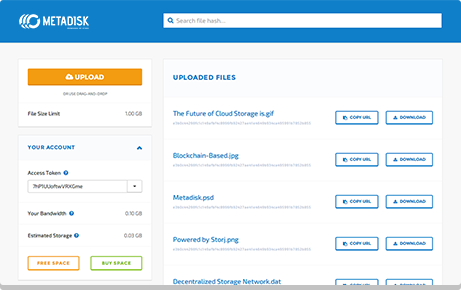
\includegraphics[width=\linewidth]{6}
\caption{Metadata Insertion into a Blockchain}
\end{figure}

Data is inserted into the blockchain via a standard transaction with extra metadata. Because this would be prohibitively expensive on the Bitcoin blockchain and not technically feasible with the strict metadata limits on its transactions, we will not use it to store this metadata. As described in the MetaDisk paper \cite{1}, we will use Florincoin \cite{6} as an initial mechanism. Eventually, we will transition to a system where we could then use the Bitcoin blockchain more directly and in a more scalable manner, through proof-of-existence \cite{4} \cite{5} \cite{7}. As blockchain technology improves we can use systems like Factom \cite{7} to provide faster throughput, and Ethereum \cite{22} to create enforceable contracts on data storage.

\section{Speed}
Increased redundancy allows for some unique features on the Storj network. Because Storj is a decentralized and distributed network, upon addition of a new farmer to the network to host a shard, we also add another peer to which we can connect to download the shard. If we set a redundancy of 20x, then we have 20 peers to download the shard from simultaneously. This is in contrast to the server-client model which relies on fast connections to the nearest data center.\\

%insert Figure 7
\begin{figure}[hbt]
\centering
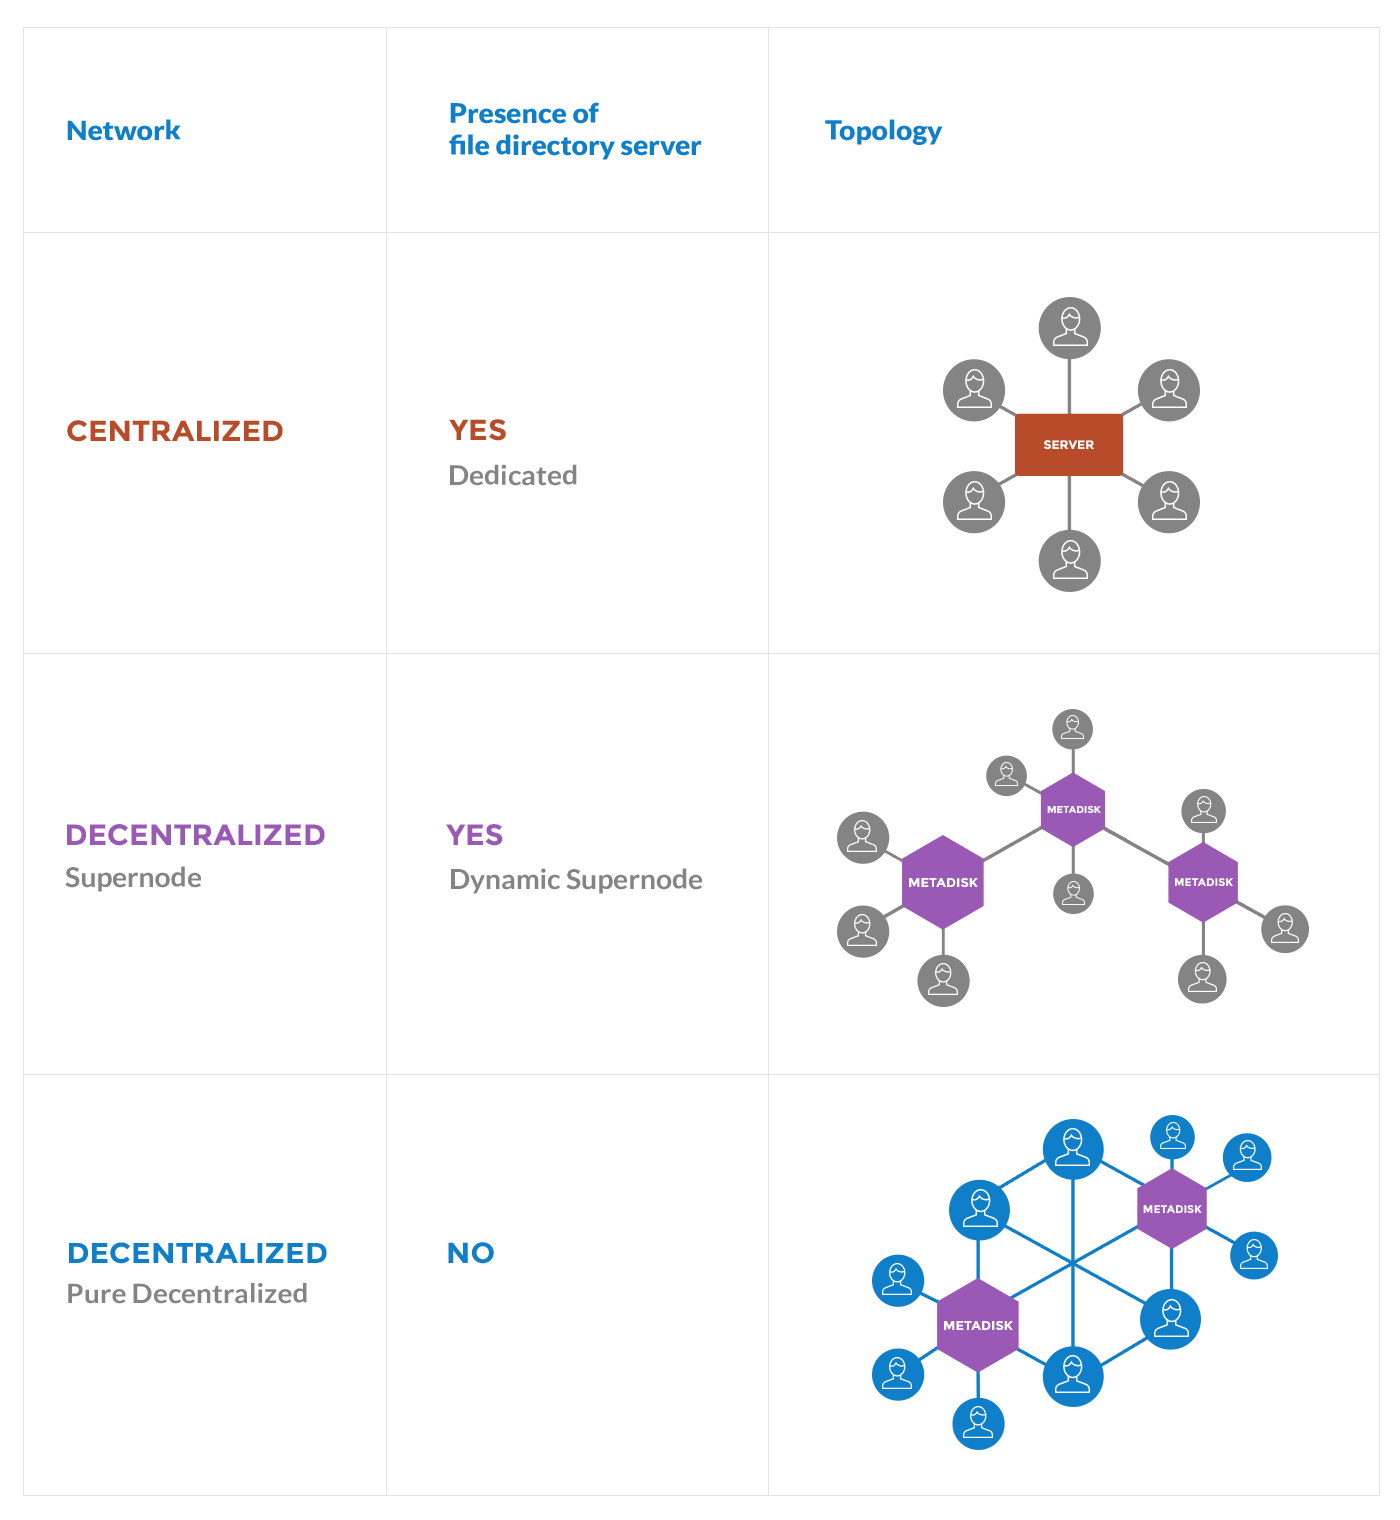
\includegraphics[width=\linewidth]{7}
\caption{Network Topology of a Server Based Network vs. a Peer-to-Peer Network}
\end{figure}

As with the standard functionality of a peer-to-peer network, we can connect to geographically close peers to achieve high transfer speeds. We can provide an incentive for peers to maintain node connectivity to the network using cryptocurrency, which solves the typical problem observed in peer-to-peer networks where there are insufficient peers for faster transfer. Although, not discussed in this paper this opens the possibility for Storj to be used as a content and data distribution method. 

\section{Rewards}
For the network to function properly we must reward the correct and agreed upon behaviors. We use the cryptocurrency Storjcoin X, or SJCX, as the baseline token for the Storj network. Clients and farmers can exchange SJCX for bandwidth and storage space on the network. \\

We can use micropayments/microtransactions \cite{12} \cite{13} to facilitate the instant transfer of cryptocurrency between nodes as payment for bandwidth or storage space. The client pays the farmer after the completion of a heartbeat. If both behave honestly and are in agreement, no further steps are necessary. Otherwise, the transaction will end and the last amount agreed upon will be considered final. We can alternately use trustless and automated mechanisms to perform disputes between nodes. As long as both parties are acting in a financially rational manner, these methods may not be necessary as the potential loss would only amount to a fraction of a cent. In the case of a targeted attack, where the attacker is only concerned with attacking the network at great financial expense, further mechanisms will be needed to protect new nodes on the network. \\

\subsection{Market Basis}
Unlike traditional cloud services that implement fixed based pricing, pricing on the Storj network is determined by the market. The efficient allocation of data resources is enabled and incentivized by the free market. Farmers are able to set asks and clients bids. Prices can vary based on bandwidth, location and speed. For example, a fast server with SSD drives might charge more than a standard home laptop. This way we can achieve efficient usage of our data sources. Bob might want to store a video file on the network for streaming. In this case Bob might want to use the fast SSD server. Alice might only be using the Storj network for backup purposes. This time the standard home laptop would serve as a cheaper and more efficient option.

\subsection{Peer Discovery}
We can get useable data on the quality and type of service of a farmer from any source, be it a tracking service or directly from the network. These are simply advertisements in peer discovery. In this way we use a pseudo-reputation system. If Bob and Alice say Eve is reputable then Eve is probably reputable. Eve might lie about uptime or speed, but our auditing mechanisms will detect this and drop Eve as a peer. In this way we are not reliant on Bob’s or Alice’s recommendation but they certainly help with finding good peers.

\subsection{Market Scale}
The market will also help balance the supply and demand of the storage space on the network. If there is an increased demand on the network for storage space, then the SJCX token will increase in value, providing an incentive for farmers to add more storage space to the network to meet demand. Likewise, as demand decreases, the storage price diminishes, slowing the growth of storage on the network. The network thus relies on the power of the market to ensure sufficient network resources. 

\subsection{Peer Rewarding}
One of the problems that exists in traditional peer-to-peer networks is insufficient peers. Peers are simply volunteers who help enable very fast transfer speeds for very popular files. By the same token, a lack of peers sharing less sought-after files often leads to painstakingly slow transfer speeds or, practically non-existent availability. Our inherent reward mechanism, based on SJCX, solves that problem by paying peers for holding shards. Using micropayments/microtransactions, we can also more directly reward peers for transferring shards to nodes that request them. This way peers may voluntarily host popular shards so that they may earn more SJCX. In a nutshell, this system enables trustless yet incentivized transfers without relying upon the technical overhead of a proof-of-bandwidth algorithm. However, a recent paper on TorPath \cite{14} has shed some light on how that might be possible. 

\subsection{Uptime}
Farmers are encouraged to have high uptime. This could be quite easy for dedicated farming hardware, but hard for the average consumer. Because of this wide variation of situations, we instead set data contracts between the client and the farmer. Therefore, each can set expectations for uptime. Bob running the farming software on his laptop could accept a data contract that allows his computer to go down periodically. However, Bob would receive a much lower rate than Alice, who has dedicated hardware and always leaves it switched on. A simple uptime monitoring service can help clients discover farmers’ uptimes. We are not inherently reliant on these uptime services. They are simply used to aid in reputable peer discovery, whereas our heartbeat algorithm more directly ensures that shards are available.

\section{Sybil and Bad Actor Attacks}
There are many types of traditional attacks that we must address in our proposed network. We list many attack types and their solutions. 
\subsection{``Google Attack''}
A “Google Attack” is a coin termed by Bitcoin Core developer Peter Todd, to describe the coordinated attack on the network by a large corporation or entity controlling vast amounts of computing power/storage space. Our research has shown that Google currently stores about 8,000 PB worth of data \cite{15}. We introduce the concept of “user space”, or the collective unused free space on the computers of average consumers. This user space could expand if users began to use Storj as their primary cloud storage platform. Our research shows that figure to be about 250,000 PB \cite{15}. Thus, even if Google suspended all of its services to attack the network, it would not be possible to outperform the resources provided by user space. We make the assertion that collective user space is greater, and will always be larger than that of the centralized cloud computing industry as a whole.

%insert Figure 8
\begin{figure}[hbt]
\centering
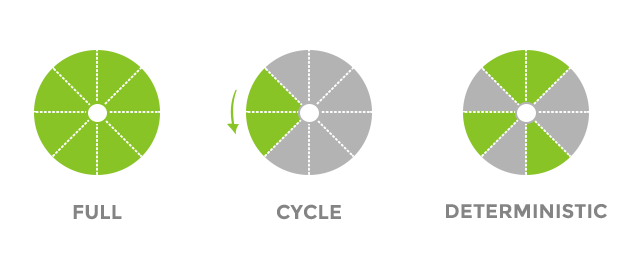
\includegraphics[width=\linewidth]{8}
\caption{Visualizing Cloud Storage vs. User Space }
\end{figure}

\subsection{Sybil Redundancy Attacks}
An attacker who would like to exploit the network by pretending that he/she has multiple redundant copies of a shard, when he/she has only one, cannot do so. This is because each shard is uniquely encrypted. Therefore, an attacker cannot pass audits unless they have copies of the unique redundant copies. The client node should take steps to distribute its redundant copies to geographically distributed and independent nodes. If randomly distributed, the probability of the same redundant piece being hosted on the same controlled node is statistically quite small. Using random distribution and our standard methods of uniquely encrypting redundant copies, an attacker cannot execute a Sybil redundancy attack.  

\subsection{Improper Distribution}
In this case we examine a malicious farmer who would like to attack the network. This attacker does not care about financial disincentives. The attacker wishes to cause distrust in the network by dropping data and its redundant copies from the network at the same time, rendering the file unrecoverable. By colluding with one or more malicious farmers, the farmer aims to receive multiple redundant copies of shard. Our first line of defence is to not use a single node when uploading a sensitive file to the network, but to instead relay shards through multiple nodes. This way, even if one of the nodes is malicious, it cannot fully carry out this attack. Nodes would have to be colluding, and if the client selects nodes randomly, the probability of selecting colluding nodes is small. Under a worst case scenario where the farmer is colluding with multiple of the relaying nodes, the second line of defense consists of two additional mechanisms. First, using erasure encoding and redundancy schemes with different parameters ensures that the farmer cannot know how many shards it needs to destroy. Furthermore we can devise a method where all verification is done on a GVN, described in section 10. With this, the farmer has no way to determine associated shards if it has multiple redundant copies. 

\subsection{Cheating Client Node}
Let us imagine a scenario whereby a malicious actor would like to host a file on the network, but avoids paying for said file, or intentionally rejects correct audits in order to avoid payment. In this case, there would be a disagreement between the two nodes, and the transaction would cease. Merkle roots embedded in the blockchain, as described previously, serve as sufficient and irrefutable proof of the validity of challenges from the client.

\subsection{Hostage Byte}
The hostage byte attack was first described by Vitalik Buterin, in which a malicious farmer transfers data to a client but holds the last piece of data “hostage” for a higher payment \cite{16}. We address this with our erasure encoding scheme, so that the shards required to reassemble the file are not linear. As long as the client keeps the bounds of its erasure encoding a secret, the malicious farmer cannot know what the last byte is.

\subsection{Honest Geppetto Attack}
In this attack vector a farmer honestly offers up a large amount of storage space for an extended period of time. At some point they “pull the strings” in an attempt to take down a large part of the network. We can make this prohibitively expensive in two ways. One, through the use of GVNs further described in Outsourceable Audits, we can delay payment to farmers. Farmers would have prove reliable for a certain amount of before starting to receive payment, and if they suddenly became malicious or unable to provide proper service the pending funds would be forfeit. Two, a bonded smart contract could be created between the client and farmer. They would both agree on a Service-level agreement(SLA) to follow, and if the farmer deviated from the agreement the client could be paid. Alternatively the funds could be destroyed.

\section{Network}
The steps to upload and retrieve a file to and from the network are:
\begin{enumerate}
\item Split the file into pieces, add erasure coding and encryption to generate shards.
\item Transfer the shards to various farmers on the network, based on distribution and erasure encoding schemes.
\item Pay each farmer upon completion of an audit.
\item The client may contact any of the farmers for data retrieval, in which case the farmers pay for the transfer of the data.
\end{enumerate}

\section{Outsourceable Heartbeats}
Traditional decentralized networks, such as Bitcoin \cite{3}, rely on consensus algorithms in order to function. They more directly use algorithms such as proof-of-work \cite{3}, in which computational power determines network consensus. Unfortunately, these mechanisms require for a majority of the nodes on the network to be honest. This has destroyed smaller cryptocurrencies such as Terracoin \cite{17} and many others, where the majority of the nodes did not behave honestly, known as a 51\% attack. Bitcoin itself has had problems with potential 51\% attacks \cite{18}. Furthermore, these algorithms waste massive amounts of computational power in order to ensure security \cite{19}, although some advancements have been made in cryptocurrencies such as Peercoin \cite{19}. \\

A 51\% attack on a standard cryptocurrency network like Bitcoin has little effect on the majority of the network. Only users transacting at the time of the attack could be defrauded, not the rest of the network. This is different for a data-based network as an attacker could alter the state of the shards of the network, and cause data loss. Depending on the data, that could have catastrophic effects on the network, and perhaps lead to its full failure. This way, we cannot rely on consensus alone to determine the state of the shards stored on the network. \\

We instead designate the client as the ultimate decision maker in the network. After all, it is the client who is paying for the storage space on the network. Using the blockchain as an irrefutable source, even though the client is the ultimate decision maker, it cannot cheat the farmer. Thanks to the auditing algorithm, it does not matter how many dishonest or colluding nodes are on the network. Malicious nodes will not be able to pass audits and unique, encrypted redundant copies will ensure that colluding nodes and Sybil attacks are not possible. \\

The question remains of how to handle audits when the client is offline. We cannot expect a traditional client to be online all of the time, so we must devise trustless methods in order to validate heartbeats and pay the farmers. We propose several methods that are individually and collectively effective methods of validation and payment. \\

\subsection{Client Controlled}
The easiest method simply involves giving clients control and access to their own online hardware. For example, they may purchase a basic VPS server for only a few dollars a month. To offset the cost, they could share it with other users or friends that they know. Operation is quite simple -- the server need only pass an audit to a farmer periodically, and verify it against a predetermined response. At the same time, it could also handle the various payments to the farmers. 

\subsection{Group of Verification Nodes}
Another method is to rely on groups of verification nodes (GVNs) that manage heartbeats and payment. A user will pass audits and payments to a GVN. In an M-of-N multisig scheme, we use N of N, where N is the number of nodes in GVN. This way, a single non-colluding and honest node is able to disprove and block payment for any colluding nodes. At the client’s discretion we may use M < N schemes. Sia \cite{20} describes some methods that could be used to eject colluding nodes. In order to ensure the client remains the ultimate decision maker, we additionally require that a transaction be crafted that returns funds to the client. This transaction would not be broadcasted, so that at any point in time the client can retrieve any unspent funds. We can further add proof-of-existence methods \cite{4} \cite{5} \cite{7} so that all actions taken by these node groups are publicly auditable through a blockchain. 

\subsection{Buried Keys}
The audit responses themselves could be the private or access keys to funds. After responding, the farmers could then redeem their keys for payment directly from the network or from a GVN. Alternately, a decentralized payment service managed by smart contracts could be a solution by itself or in concert with a GVN. 

\subsection{Dust and Anonymizing}
GVNs allow us to collate millions of verifications and payments into singular payments to the farmers. Ideally, the GVN and farmer would establish a micropayments channel, and the farmer would be paid via the GVN instantly per verification. This would allow us to avoid making millions of small dust transactions. Furthermore, a GVN will provide anonymity to the users, as funds can be mixed within it. Therefore, there is no direct or indirect link between a user’s funds and their files.

\subsection{Extending GVNs}
As we lay out the ideas for Storj, there are several other methods being developed that could handle audits and trustless payments. These include Factom \cite{7}, oracles \cite{21}, smart contracts, Turing-complete blockchains [22], P2P networks, blockchains, quorums \cite{20}, and scratch-off puzzles \cite{23}. Each one of these methods could be a useful and trustless method of handling heartbeats and payments. While MetaDisk \cite{1} will serve as the first implementation of a node in a GVN, these other methods could also serve as nodes in a GVN. Our core goal is to have the client as the ultimate decider. The client can either handle these tasks, or have full power over which algorithms the client feels most comfortable with protecting its data. 

%insert figure 10
\begin{figure}[hbt]
\centering
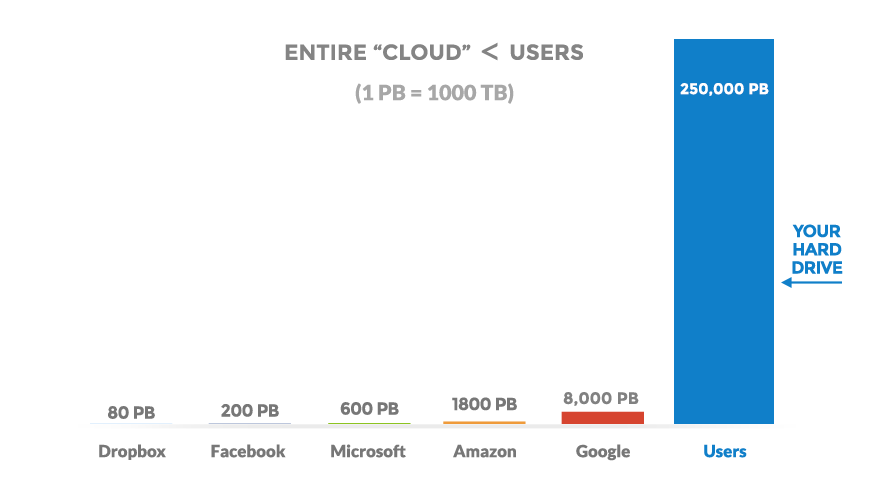
\includegraphics[width=\linewidth]{9}
\caption{Visualizing an Example of GVN}
\end{figure}

\section{Calculations}
The chance of failure of k-of-n erasure coding failing assuming probability p every shard stays online, is calculated as follows:

\vspace{2cm}
{\centering
$\Pr_{failure}(n,k,p) = \displaystyle \sum_{i=0}^{k-1} p^{k}(1-p)^{n-k }{n \choose k}$
\\}
\vspace{3cm}
%code formatting
\begin{table}[hbt!]
\begin{center}
\begin{tabular}{r r l r}
n & k & p & $\Pr_{failure}{n,k,p}$\\
\hline  9&  3&    0.5  &  8.984e-02 \\
\hline  9&  3&    0.75& 1.342e-03\\
\hline  9&  3&    0.9  &  2.998e-06\\
\hline  9&  3&    0.98& 4.448e-11\\
\hline  9&  2&    0.5  &  1.953e-02\\
\hline  9&  2&    0.75& 1.068e-04\\
\hline  9&  2&    0.9  &  8.200e-08\\
\hline  9&  2&    0.98& 2.263e-13\\
\hline  18& 6&   0.5  & 4.812e-02\\
\hline  18& 6&   0.75&3.424e-05\\
\hline  18& 6&   0.9  & 5.266e-10\\
\hline  18& 6&   0.98&6.391e-19\\
\hline  18& 4&   0.5  & 3.768e-03\\
\hline  18& 4&   0.75&3.414e-07\\
\hline  18& 4&   0.9  & 6.074e-13\\
\hline  18& 4&   0.98&2.526e-23\\
\hline  36& 12& 0.5  &1.440e-02\\
\hline  36& 12&  0.75&2.615e-08\\
\hline  36& 12&  0.9  &1.977e-17\\
\hline  36& 12&  0.98&1.628e-34\\
\hline  36&  8&   0.5  & 1.562e-04\\
\hline  36& 8&   0.75 &4.187e-12\\
\hline  36& 8&   0.9  & 4.098e-23\\
\hline  36& 8&   0.98 &3.909e-43\\
\hline  72& 24& 0.5  &1.471e-03\\
\hline  72& 24& 0.75&1.937e-14\\
\hline  72& 24& 0.9  &3.636e-32\\
\hline  72& 24& 0.98&1.390e-65\\
\hline  72& 16& 0.5  &3.269e-07\\
\hline  72& 16& 0.75&8.130e-22\\
\hline  72& 16& 0.9  &2.449e-43\\
\hline  72& 16& 0.98&1.236e-82\\
\hline  
\end{tabular}
\end{center}
\end{table}

%code formatting
Code:
\begin{lstlisting}
def fac(n): return 1 if n==0 else n * fac(n-1)
def choose(n,k): return fac(n) / fac(k) / fac(n-k) 
def prob(n,k,p): return choose(n,k) * p ** k * (1-p) ** (n-k)
def prob\_fail(n,k,p): return sum([prob(n, i, p) for i in range(0, k)])
\end{lstlisting}
Therefore, with sufficient parameters for erasure encoding, in addition to recovery methods described above, the statistical chance of shard or file loss is quite small. 


\section{Conclusion}
We have outlined a peer-to-peer cloud storage network implementing end-to-end encryption which allows users to transfer and share data without reliance on a third party data provider. We have addressed problems such as Sybil attacks and peer disconnects by using uniquely encrypted redundant copies, and an audit algorithm which periodically checks for file availability and integrity. By using cryptocurrency, we can provide the proper incentives for growth of the network and the trading of data between a client and farmer. We give the client full power over the algorithms that handle verification and payments for their files. Using these methods, we hand back control of cloud data to the users. \\

We also postulate that in the absence of a peer-to-peer network the described methods may be used to allow users to control, migrate and validate their data on 3rd party data providers. In essence, running a trustless and failure-tolerant system on trusted data providers greatly increases security and privacy.\\




\bibliographystyle{unsrt}
\begingroup
  \raggedright
  \bibliography{storj}
\endgroup


\end{document}
